\documentclass[xcolor=svgnames]{beamer}
\usepackage{tikz}
\usepackage[utf8]{inputenc}
\usepackage{xcolor}
\usepackage{booktabs, comment} 
\usepackage{pgfpages}
\usepackage{csquotes}
\usepackage{amsmath}
\usepackage{caption}
\usepackage{hyperref}
\usepackage{biblatex}
\usepackage{array}
\usepackage{algorithm}
\usepackage{algpseudocode}

\usetheme{Madrid}
% COLORS 
\definecolor{mqred}{RGB}{166, 25, 46}
\definecolor{mqdeepred}{RGB}{118, 35, 47}
\definecolor{mqgray}{RGB}{55, 58, 54}
\definecolor{mqlightgray}{RGB}{237, 235, 229}
\definecolor{mqmagenta}{RGB}{198, 0, 126}
\usecolortheme[named=mqred]{structure}
\setbeamercolor{title in head/foot}{bg=mqlightgray, fg=mqgray}
\setbeamercolor{author in head/foot}{bg=mqdeepred}
\setbeamercolor{page number in head/foot}{bg=mqdeepred, fg=mqlightgray}

\setbeamersize{text margin left=0.8cm, text margin right=0.8cm}
% FOOTNOTE ARRANGEMENTS

\usetikzlibrary{positioning}
\makeatletter
\setbeamertemplate{footline}{
  \leavevmode%
  \hbox{%
  \begin{beamercolorbox}[wd=.5\paperwidth,ht=3ex,dp=2ex,center]{author in head/foot}%
    \usebeamerfont{author in head/foot}\insertshortauthor\expandafter\ifblank\expandafter{\beamer@shortinstitute}{}{~~(\insertshortinstitute)}
  \end{beamercolorbox}%
  \begin{beamercolorbox}[wd=.4\paperwidth,ht=3ex,dp=2ex,center]{title in head/foot}%
    \usebeamerfont{title in head/foot}\insertshorttitle
  \end{beamercolorbox}%
  \begin{beamercolorbox}[wd=.1\paperwidth,ht=3ex,dp=2ex,center]{page number in head/foot}%
    \usebeamerfont{page number in head/foot}\insertframenumber{} / \inserttotalframenumber 
  \end{beamercolorbox}}%
  \vskip0pt%
}
\makeatother
\beamertemplatenavigationsymbolsempty
\setbeamertemplate{enumerate item}{\textbf{\insertenumlabel.}}
%% ******************************************* added <<<<<<<<<<<<<<
\newcounter{enumstate}
\stepcounter{enumstate}

\newcommand{\Staten}{\item[\textbf{Step \theenumstate:}]\stepcounter{enumstate}}% numbered state with dot
\algnewcommand\algorithmicforn{\hspace*{-3ex}\textbf{Step \theenumstate:}\stepcounter{enumstate} \ \textbf{for}} % numbered for with dot
\algdef{SE}[FOR]{Forn}{EndForn}[1]{ \algorithmicforn\  #1\ \algorithmicdo}{\algorithmicend\ \algorithmicfor}%   
\algnewcommand\algorithmicifn{\hspace*{-2.75ex}\textbf{Step \theenumstate:} \stepcounter{enumstate} \textbf{if}} % Numbered if with 'Step' and bold
\algdef{SE}[IF]{Ifn}{EndIfn}[1]{\algorithmicifn\ #1\ \algorithmicthen}{\algorithmicend\ \algorithmicif}% Custom if environment
%% *******************************************
\AtBeginSection[]
{
  \begin{frame}{Table of Contents}
    \tableofcontents[currentsection]
  \end{frame}
}
% TITLE, AUTHORS, INSTITUTE, DATE

\title[Combinatorial Rounding] 
{Combinatorial Rounding}
\subtitle{Section 7.3}
\author[Wasif Hamid] % (optional)
{1905026 - Wasif Hamid }

\institute[CSE, BUET] % (optional)
{
  Department of Computer Science and Engineering\\
  Bangladesh University of Engineering and Technology
}

\date[17 Nov 2024] % (optional)
{17 November 2024}


% LOGO
\titlegraphic{\includegraphics[height=1.75cm]{BUET_LOGO.svg.png}} 

\addbibresource{ref.bib}
\begin{document}

\frame{\titlepage}

\begin{frame}{Presentation Outline}
    \tableofcontents
\end{frame}
\begin{section}{Introduction}
    \begin{frame}{Combinatorial Rounding}
        \begin{itemize}[<+->]
            \item To efficiently solve Integer Linear Programs, we can relax them into linear programs that permit real values, making them easier to solve. However, this may result in non-feasible solutions. 
            \item Combinatorial Rounding applies various rounding strategies to convert these optimal real-valued solutions into integer values, yielding feasible solutions that also provide good approximation ratios.
        \end{itemize}
    \end{frame} 
\end{section}
\begin{section}{Minimum Weight Vertex Cover}
    \begin{frame}{Minimum Weight Vertex Cover}
        A vertex cover problem with weights on vertices and we need to minimize the weight of the solution set. For a graph $G=(V,E)$ the ILP version of the problem can be defined below- 
        \begin{block}{Min-WVC Integer Linear Program}
            \[
                \begin{array}{lll}
                \text{Minimize} & w_1 x_1 + w_2 x_2 + \cdots + w_n x_n \\[10pt]
                \text{Subject to} & x_i + x_j \geq 1, \quad & \text{for each }\{v_i, v_j\} \in E \\[10pt]
                & x_i = 0 \text{ or } 1, \quad & i = 1, 2, 3, \dots, n
                \end{array}
            \]
        \end{block}
        \pause
        \begin{exampleblock}{Relaxation to Linear Program}
            \[
                x_i = 0 \text{ or } 1 \quad \xrightarrow{\text{relaxation}} \quad 0 \leq x_i \leq 1
            \]
        \end{exampleblock}
    \end{frame}
    \begin{frame}{Example}
        \begin{minipage}
            {0.45\textwidth}
            \centering
            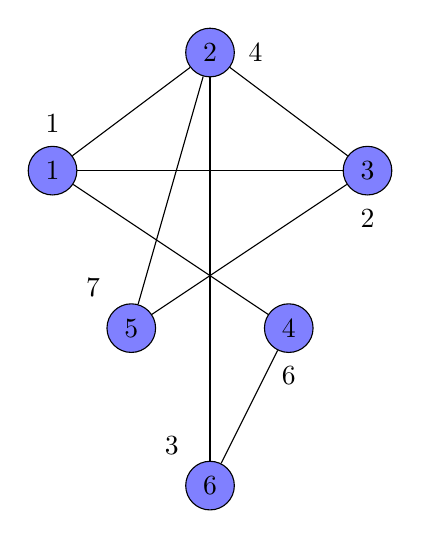
\begin{tikzpicture}
                % Nodes
                \node[circle, draw, fill=blue!50] (1) at (0, 0) {1};   % Internal node
                \node[circle, draw, fill=blue!50] (2) at (2, 1.5) {2}; % Internal node
                \node[circle, draw, fill=blue!50] (3) at (4, 0) {3}; % Leaf
                \node[circle, draw, fill=blue!50] (4) at (3, -2) {4}; % Leaf
                \node[circle, draw, fill=blue!50] (5) at (1, -2) {5}; % Leaf
                \node[circle, draw, fill=blue!50] (6) at (2, -4) {6}; % Leaf

                \node[above=0.05cm of 1] {$1$};
                \node[right=0.05cm of 2] {$4$};
                \node[below=0.05cm of 3] {$2$};
                \node[below=0.05cm of 4] {$6$};
                \node[above left=0.05cm and 0.05cm of 5] {$7$};
                \node[above left=0.05cm and 0.05cm of 6] {$3$}; 
                % Edges
                \draw (1) -- (2);
                \draw (1) -- (3);
                \draw (1) -- (4);
                \draw (2) -- (5);
                \draw (2) -- (3);
                \draw (2) -- (6);
                \draw (3) -- (5);
                \draw (4) -- (6);
            \end{tikzpicture}
        \end{minipage}
        \hfill
        \pause
        \begin{minipage}
            {0.45\textwidth}
            \centering
            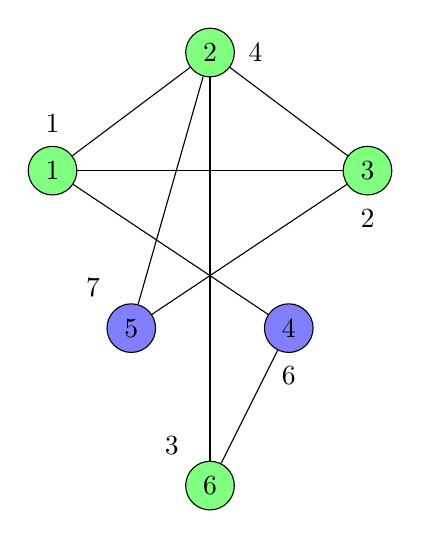
\begin{tikzpicture}
                % Nodes
                \node[circle, draw, fill=green!50] (1) at (0, 0) {1};   % Internal node
                \node[circle, draw, fill=green!50] (2) at (2, 1.5) {2}; % Internal node
                \node[circle, draw, fill=green!50] (3) at (4, 0) {3}; % Leaf
                \node[circle, draw, fill=blue!50] (4) at (3, -2) {4}; % Leaf
                \node[circle, draw, fill=blue!50] (5) at (1, -2) {5}; % Leaf
                \node[circle, draw, fill=green!50] (6) at (2, -4) {6}; % Leaf

                \node[above=0.05cm of 1] {$1$};
                \node[right=0.05cm of 2] {$4$};
                \node[below=0.05cm of 3] {$2$};
                \node[below=0.05cm of 4] {$6$};
                \node[above left=0.05cm and 0.05cm of 5] {$7$};
                \node[above left=0.05cm and 0.05cm of 6] {$3$}; 
                
                % Edges for spanning tree
                \draw (1) -- (2);
                \draw (1) -- (3);
                \draw (1) -- (4);
                \draw (2) -- (5);
                \draw (2) -- (3);
                \draw (2) -- (6);
                \draw (3) -- (5);
                \draw (4) -- (6);
            \end{tikzpicture}
        \end{minipage}
        \vspace{15pt}
        \captionof{figure}{Minimum Weight Vertex Cover}
    \end{frame}
    \begin{frame}{Linear Programming Approximation Algorithm for Min-WVC}
        \textbf{Input:} A graph \( G = (V, E) \) and a weight function \( w : V \rightarrow \mathbb{N} \).
        
        \begin{enumerate}
            \item Convert the input into a 0-1 integer program, and construct the corresponding linear program.
            \item Find an optimal solution \( x^* \) to the linear program (7.12).
            \item For \( i = 1, 2, \dots, n \):
            \[
            x^A_i = 
            \begin{cases} 
              1, & \text{if } x^*_i \geq \frac{1}{2}, \\ 
              0, & \text{otherwise.} 
            \end{cases}
            \]
            \item Output \( x^A \).
        \end{enumerate}
    \end{frame}

% Slide 2: 2-Approximation Proof
    \begin{frame}{2-Approximation Ratio Proof}
        For each \( \{v_i, v_j\} \in E \):
        
        \[
        x^*_i + x^*_j \geq 1 \Rightarrow \text{at least one of } x^*_i \text{ or } x^*_j \geq \frac{1}{2}.
        \]
        \pause
        This implies that at least one of \( x^A_i \) or \( x^A_j \) is equal to 1, so \( x^A \) is a feasible solution to the integer program.
        
        \vspace{0.3cm}
        \pause
        Furthermore,
        \[
        \sum_{i=1}^n w_i x^A_i \leq 2 \sum_{i=1}^n w_i x^*_i.
        \]
        
        This shows that the cost of \( x^A \) is at most twice the cost of the optimal solution \( x^* \) to the linear program.
        
        \vspace{0.3cm}
        \pause
        Therefore the proposed algorithm is a \textbf{polynomial-time 2-approximation} for Min-WVC.
    \end{frame}
    \begin{frame}{Example}
        \begin{minipage}
            {0.45\textwidth}
            \centering
            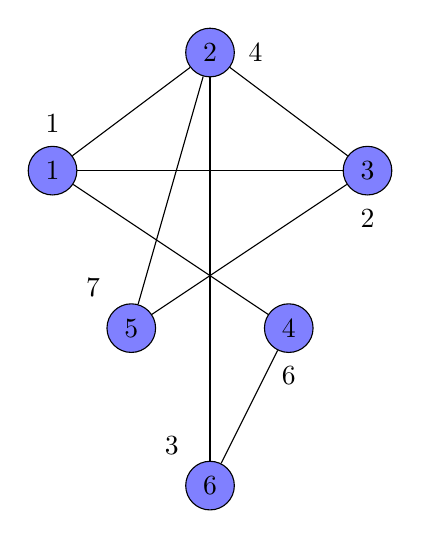
\begin{tikzpicture}
                % Nodes
                \node[circle, draw, fill=blue!50] (1) at (0, 0) {1};   % Internal node
                \node[circle, draw, fill=blue!50] (2) at (2, 1.5) {2}; % Internal node
                \node[circle, draw, fill=blue!50] (3) at (4, 0) {3}; % Leaf
                \node[circle, draw, fill=blue!50] (4) at (3, -2) {4}; % Leaf
                \node[circle, draw, fill=blue!50] (5) at (1, -2) {5}; % Leaf
                \node[circle, draw, fill=blue!50] (6) at (2, -4) {6}; % Leaf

                \node[above=0.05cm of 1] {$1$};
                \node[right=0.05cm of 2] {$4$};
                \node[below=0.05cm of 3] {$2$};
                \node[below=0.05cm of 4] {$6$};
                \node[above left=0.05cm and 0.05cm of 5] {$7$};
                \node[above left=0.05cm and 0.05cm of 6] {$3$}; 
                % Edges
                \draw (1) -- (2);
                \draw (1) -- (3);
                \draw (1) -- (4);
                \draw (2) -- (5);
                \draw (2) -- (3);
                \draw (2) -- (6);
                \draw (3) -- (5);
                \draw (4) -- (6);
            \end{tikzpicture}
        \end{minipage}
        \hfill
        \pause
        \begin{minipage}
            {0.45\textwidth}
            \centering
            \textbf{Objective:}
            \\
            $Z=x_1+4x_2+2x_3+6x_4+7x_5+3x_6$
            \\
            \vspace{5pt}
            \\
            \textbf{Constraints:}
            \\
            $x_1+x_2\geq1,$\\
            $x_1+x_3\geq1,$\\
            $x_1+x_4\geq1,$\\
            $x_2+x_3\geq1,$\\
            $x_2+x_5\geq1,$\\
            $x_2+x_6\geq1,$\\
            $x_3+x_5\geq1$\\
            $x_4+x_6\geq1$\\
            $x_1,x_2,x_3,x_4,x_5,x_6\geq0$
        \end{minipage}
    \end{frame}
    \begin{frame}{Example(Cont.)}
        \begin{minipage}
            {0.45\textwidth}
            Solving the linear program we get the following:
            \begin{center}
                $min(Z)=10$ \\ for \\ $x^*=[1,1,1,0,0,1]$\\
            \end{center}
            The solution is already integers so we do not need to round up or down.\\
            \\
            So, the solution set is 
            \begin{center}
                $C=\{1,2,3,6\}$
            \end{center}
            
        \end{minipage}
        \hfill
        \pause
        \begin{minipage}
            {0.45\textwidth}
            \centering
            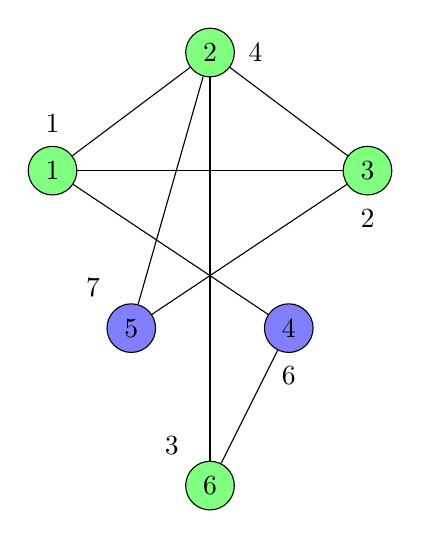
\begin{tikzpicture}
                % Nodes
                \node[circle, draw, fill=green!50] (1) at (0, 0) {1};   % Internal node
                \node[circle, draw, fill=green!50] (2) at (2, 1.5) {2}; % Internal node
                \node[circle, draw, fill=green!50] (3) at (4, 0) {3}; % Leaf
                \node[circle, draw, fill=blue!50] (4) at (3, -2) {4}; % Leaf
                \node[circle, draw, fill=blue!50] (5) at (1, -2) {5}; % Leaf
                \node[circle, draw, fill=green!50] (6) at (2, -4) {6}; % Leaf

                \node[above=0.05cm of 1] {$1$};
                \node[right=0.05cm of 2] {$4$};
                \node[below=0.05cm of 3] {$2$};
                \node[below=0.05cm of 4] {$6$};
                \node[above left=0.05cm and 0.05cm of 5] {$7$};
                \node[above left=0.05cm and 0.05cm of 6] {$3$}; 
                
                % Edges for spanning tree
                \draw (1) -- (2);
                \draw (1) -- (3);
                \draw (1) -- (4);
                \draw (2) -- (5);
                \draw (2) -- (3);
                \draw (2) -- (6);
                \draw (3) -- (5);
                \draw (4) -- (6);
            \end{tikzpicture}
        \end{minipage}
        \vspace{15pt}
    \end{frame}
\end{section}
\begin{section}{Minimum 2-Satisfiability}
    \begin{frame}{Minimum 2-Satisfiability}
        \small
        \begin{block}{Problem Statement}
            Given a Boolean formula in 2-CNF, determine whether it is satisfiable and, if it is, find a satisfying assignment that contains a minimum number of true variables.
        \end{block}
        \begin{exampleblock}{Min-2SAT Linear Program}
            \[
                \begin{array}{lll}
                    \text{Minimize} & x_1 +  x_2 +  x_3 + \cdots + x_n \\[10pt]
                    \text{Subject to} & x_i + x_j \geq 1, \quad \quad \quad \quad \quad & \text{for each clause}\{x_i\lor x_j\} \text{ in } F \\[10pt]
                    & (1-x_i )+ x_j \geq 1, \quad \quad & \text{for each clause}\{\bar{x}_i\lor x_j\} \text{ in } F \\[10pt]
                    & (1-x_i) + (1-x_j) \geq 1, & \text{for each clause}\{\bar{x}_i\lor \bar{x}_j\} \text{ in } F \\[10pt]
                    & 0 \leq x_i \leq  1, \quad & i = 1, 2, 3, \dots, n
                
                \end{array}
            \]
        \end{exampleblock}
    \end{frame}
    \begin{frame}{Linear Programming Approximation Algorithm for Min-2SAT}
    \small
    \begin{algorithmic}
    \begin{columns}
        \begin{column}
            {0.4\textwidth}
            \setcounter{enumstate}{1}
            \Staten Convert formula $F$ into a linear program and find an optimal solution $x^*$ for it.
            \Forn{$i \gets 1$ to $n$}
                \If{$x^*_i > \frac{1}{2}$}
                    \State $x^A_i \gets 1$
                \ElsIf{$x^*_i < \frac{1}{2}$}
                    \State $x^A_i \gets 0$
                \EndIf
            \EndFor
        \end{column}
        \pause
        \begin{column}
            {0.45\textwidth}
            \setcounter{enumstate}{3}
            \Staten Let $F_1$ be the collection of all clauses both of whose two variables have $x^*$ value equal to $\frac{1}{2}$, and let $J \gets \{j \mid 1 \leq j \leq n, x_j \text{ is in } F_1\}$.
            \Forn{$i \gets 1$ to $n$}
                \If{$x^*_i = \frac{1}{2}$ and $i \notin J$}
                    \State $x^A_i \gets 0$
                \EndIf
            \EndFor
        \end{column}
        \end{columns}
        \pause
        \vspace{10pt}
            \Ifn{$F_1$ is satisfiable}
                \State Let $x^A_J$ be a satisfying assignment for $F_1$ and output $x^A$.
            \Else
                \State Output ``$F$ is not satisfiable.''
            \EndIf
        \end{algorithmic}
    \end{frame}
    \begin{frame}{Satisfiability and Performance Ratio of the algorithm}
        \begin{block}{Satisfiability of Clauses}
            \begin{itemize}
                \item By step (5), every clause in $F_1$ is satisfied by $x^A$.
                \item For a clause $(x_i \lor x_j)$ not in $F_1$:
                \begin{itemize}
                    \item $x^*_i + x^*_j \geq 1$ implies $x^*_i > \frac{1}{2}$ or $x^*_j > \frac{1}{2}$.
                    \item By step (2), either $x^A_i = 1$ or $x^A_j = 1$, ensuring the clause $(x_i \lor x_j)$ is satisfied.
                \end{itemize}
                \item The same reasoning applies to other types of clauses, such as $(x_i \lor \bar{x}_j)$ or $(\bar{x}_i \lor \bar{x}_j)$.
            \end{itemize}
        \end{block}
        
        \vspace{0.5cm}
        \pause
        \begin{exampleblock}{Performance Ratio}
            \begin{itemize}
                \item For each $i = 1, 2, \ldots, n$, we have $x^A_i \leq 2x^*_i$.
                \item Thus, $x^A$ is an approximation with a performance ratio $\leq 2$.
            \end{itemize}
        \end{exampleblock}
    \end{frame}
    \begin{frame}{Polynomial 2-SAT Algorithm}
    
        \textbf{Input:} A 2-CNF formula $F_1$ over variables $x_1, x_2, \ldots, x_n$.

        \begin{enumerate}
            \item<1-> Construct a digraph $G(F_1) = (V, E)$ as follows:
            \[
            V \gets \{x_i, \bar{x}_i \mid 1 \leq i \leq n\},
            \]
            \[
            E \gets \{(\neg y_i, y_j), (\neg y_j, y_i) \mid (y_i \lor y_j) \text{ is a clause in } F_1\},
            \]
            where $y_i$ denotes a literal $x_i$ or $\bar{x}_i$.
            \only<2>{
                \begin{figure}
                    \centering
                    \includegraphics[width=.5\linewidth]{graph.png}
                    \caption{\centering Digraph for \( F_1 = (\lnot x_1 \lor x_2) \land (\lnot x_2 \lor \lnot x_3) \land (\lnot x_1 \lor x_3) \land (x_3 \lor \lnot x_4) \land (x_1 \lor \lnot x_4) \)}
                \end{figure}
                
            }
            \item<3-> \textbf{For} $i \gets 1$ to $n$ \textbf{do}
            \begin{itemize}
                \item[] \textbf{If} vertices $x_i$ and $\bar{x}_i$ are strongly connected, \textbf{then} output ``$F_1$ is not satisfiable'' and halt.
            \end{itemize}
            
            \item<4-> \textbf{For} $i \gets 1$ to $n$ \textbf{do}
            \begin{itemize}
                \item \textbf{If} there is a path from $x_i$ to $\bar{x}_i$, \textbf{then} for each literal $y_j$ that is reachable from $\bar{x}_i$, set $\tau(y_j) \gets 1$.
                \item \textbf{If} there is a path from $\bar{x}_i$ to $x_i$, \textbf{then} for each literal $y_j$ that is reachable from $x_i$, set $\tau(y_j) \gets 1$.
            \end{itemize}
            
            \item<5-> \textbf{For} $i \gets 1$ to $n$ \textbf{do}
            \begin{itemize}
                \item \textbf{If} $\tau(x_i)$ is undefined, \textbf{then} for each literal $y_j$ that is reachable from $x_i$, set $\tau(y_j) \gets 1$.
            \end{itemize}
            
            \item<6-> \textbf{Output} $\tau$.
        \end{enumerate}
    
    \end{frame}

    \begin{frame}{Example of 2-SAT Assignment}
        \small
        \begin{figure}
            \centering
            \includegraphics[width=0.5\linewidth]{graph.png}
            \label{fig:enter-label}
        \end{figure}
        \begin{itemize}
            \item<1-> Given \( F_1 = (\bar{x}_1 \lor x_2) \land (\bar{x}_2 \lor \bar{x}_3) \land (\bar{x}_1 \lor x_3) \land (x_3 \lor \bar{x}_4) \land (x_1 \lor \bar{x}_4) \), we constructed the above digraph.
            \item<2> None of any $x_i$ and $\bar{x}_i$ pair are strongly connected. So we continue to step 3.
            \vspace{-2.5em}
            \item<3> At the start $\tau=[-,-,-,-]$
            \only<3>{
                \begin{itemize}
                    \small
                    \item $\bar{x}_1$ is reachable from $x_1$.
                    \item $\bar{x}_4$ is reachable from $\bar{x}_1$:
                    \item Using Step 3.1, Set \(\bar{x}_4 = 1\), so \(x_4 = 0\).
                    \item No other negation of a literal reachable from itself gives us more assignments.
                \end{itemize}
            }
            \vspace{-2.5em}
            \item<4> After previous step $\tau=[-,-,-,0]$
            \only<4>{
                \begin{itemize}
                    \small
                    \item $x_1$ is still undefined.
                    \item $x_2,\bar{x}_3,\bar{x}_1$ is reachable from $x_1$:
                    \item Set \(x_2 = 1\), $\bar{x}_3=1$ and $\bar{x}_1=1$, so we get \(x_2=1,x_3=0 \text{ and }x_4 = 0\).
                \end{itemize}
            }
            \vspace{-2.5em}
            \item<5-> Resulting assignment:
            \[
            \tau(x_1) = 0, \quad \tau(x_2) = 1, \quad \tau(x_3) = 0, \quad \tau(x_4) = 0
            \]
            \item<5-> This assignment satisfies all the clauses in $F_1$ 
        \end{itemize}
    \end{frame}
\begin{frame}{Correctness of the Algorithm}
    \begin{itemize}
        \item<1->   
        If there is an edge \((y, z)\) in \(E\), any satisfying assignment \(\tau\) must satisfy:  
        \[
        \tau(y) = 1 \implies \tau(z) = 1.
        \]
        \item<2-> 
        This property extends to all pairs \(y, z\) where there is a path from \(y\) to \(z\).
        \item<3-> Thus, if any variable \(x_i\) and its negation \(\bar{x}_i\) are in the same strongly connected component \(F_1\) is \textbf{unsatisfiable}. So, the Algorithm terminates correctly in Step (2).
        \item<4-> If there is a path from \(y \to z\), then there is a path from \(\bar{z} \to \bar{y}\). This ensures that no variable is assigned both 1 and 0 at the same time in step 3 and step 4.
        \only<5-7>
        {
        \begin{itemize}
            \item<5-7> Suppose a variable $w$ is assigned both. So, $\tau(w)=1$, so there must be path $\bar{u} \rightarrow {u} \rightarrow w $. So there must be a path from $\bar{w}$ to $\bar{u}$.
            \item<6-7> Again, $\tau(\bar{w})=1$, so there must be path $\bar{v} \rightarrow v \rightarrow \bar{w} $. So there must be a path from ${w}$ to $\bar{v}$.
            \item<7> So we get a path, $w\rightarrow \bar{v} \rightarrow \bar{w} \rightarrow \bar{u} \rightarrow w$ which is a cycle. If that exists step 2 would have already discarded the problem.
        \end{itemize}
        }
        \item<8-> Each clause $(y_i \lor y_j )$ in $F_1$ generates two edges $(\bar{y}_i, y_j)$ and $(\bar{y}_j , y_i)$ in $E$. From steps (3) and (4), we see that it is not possible to assign $\tau (y_i) = \tau (y_j )=0$ 
        \item <9> $\tau$ must be a satisfying assignment for $F_1$.
    \end{itemize}
\end{frame}

\end{section}
\begin{section}{Scheduling on Unrelated Parallel Machines}
    \small
    \begin{frame}{Scheduling on Unrelated Parallel Machines}
        \begin{block}{Problem Statement}
            Given $n$ jobs, $m$ machines and, for each $1 \leq i \leq m$ and each $1 \leq j \leq n$, the amount of time $t_{ij}$ required for the $i$th machine to process the $j$th job, find the schedule for all $n$ jobs on these $m$ machines that minimizes the maximum processing time over all machines.
        \end{block}
        \pause
        \begin{exampleblock}{SCHEDULE-UPM Linear Program}
        \[
            \begin{aligned}
                \text{Minimize } & \; \quad t \\
                \text{Subject to} & \; \quad \sum_{i=1}^m x_{ij} = 1, &\; 1\leq j \leq n, \\
                & \; \quad  \sum_{j=1}^n x_{ij} t_{ij} \leq t,& \; 1\leq i \leq m, \\
                & \; \quad  0\leq x_{ij} \leq 1, &\; 1\leq i \leq m,  1\leq j \leq n.
            \end{aligned}
            \]
        \end{exampleblock}
    \end{frame}
\begin{frame}{Rounding Using Bipartite Graphs}
    \begin{itemize}[<+->]
        \item Let \(J = \{j \mid 0 < x_{ij}^* < 1\}\) and \(M = \{1, \dots, m\}\).
        \item Define \(H = (M, J, E)\), where:
        \[
        E = \{(i, j) \mid 0 < x_{ij}^* < 1\}.
        \]
        \item We need to show, $H$ contains a matching covering $J$.For that, it suffices to show each connected component of $H$ contains a matching covering all jobs in the component.
        \item Consider a connected component $H' = (M', J', E')$ of $H$.
        \item Fix $x_{ij} = x^*_{ij}$ for $i \notin M'$ or $j \notin J'$.
        \item Remaining variables form a new LP with extreme point \[x' = (x^*_{ij})_{i \in M', j \in J'}\].
        \vspace{-1.5em}
        \item $x'$ is determined by $|M'||J'|$ active constraints(constraint that are at equality).
        \item At most $|M'| + |J'|$ non-integral components, implying $H'$ has at most $ |M'| + |J'|$ edges.
    \end{itemize}
\end{frame}
\begin{frame}{Matching in $H'$}
    \textbf{Case 1: $H'$ is a Tree}
    \begin{itemize}
        \item Root the tree at any vertex $r \in J'$.
        \item A vertex $j \in J'$ cannot be a leaf, as $\sum_{i \in M'} x_{ij} = 1$ implies at least two edges incident on $j$.
        \item For each $j \in J'$, match it to one of its children.
    \end{itemize}
    \pause
    \textbf{Case 2: $H'$ is a Tree Plus an Edge}
    \begin{itemize}
        \item The extra edge forms a cycle and $H'$ is the cycle plus some trees growing out.
        \item Match all vertices on the cycle.(This is always possible as $H'$ is bipartite guaranteeing even length cycle).
        \item Contract the cycle into a root point $\rightarrow$ remaining graph becomes a tree.
        \item Match internal vertices as in Case 1.
    \end{itemize}
    
\end{frame}


\begin{frame}{Final Approximation Strategy}
\textbf{Steps:}
\begin{itemize}
    \item Assign jobs with \(x_{ij}^* = 1\) directly to machine \(i\).
    \item For partially assigned jobs, find a matching in \(H\) and assign jobs accordingly.
\end{itemize}
\pause
\textbf{Approximation Bound:}
    \[
        \text{Makespan } \leq \text{opt} + \max_{1 \leq i \leq m, 1 \leq j \leq n} t_{ij},
    \]
    where $\text{opt}$ is the minimum makespan. But we can't bound $\max t_{ij}$ by a constant times $\text{opt}$ as it can be much greater than opt.\\
    \pause
    \vspace{5pt}
    \textbf{Observation:} If $t_{ij} > \text{opt}$, job $j$ cannot be assigned to machine $i$ in the optimal solution. Therefore, we can prune the variable $x_{ij}$ from the LP, and expect to get the same solution
\end{frame}
\begin{frame}{Pruning and LP-Based Approximation}
    \begin{itemize}[<+->]
        \item If $t_{ij} > T$, remove the variable $x_{ij}$ from the LP effectively creating a bound $T$ to find feasible solutions while ensuring $T \geq \text{opt}$.
        \item Solve the following LP (7.16) to find the minimum $T$:
        \[
            \begin{aligned}
                \text{Minimize } & \; \quad t \\
                \text{Subject to} & \; \quad \sum_{1 \leq i \leq m, t_{ij} \leq T} x_{ij} = 1, &\; 1\leq j \leq n, \\
                & \; \quad  \sum_{1 \leq j \leq n, t_{ij} \leq T} x_{ij} t_{ij} \leq t,& \; 1\leq i \leq m, \\
                & \; \quad  0\leq x_{ij} \leq 1, &\; 1\leq i \leq m,  1\leq j \leq n.
            \end{aligned}
            \]
        \item Use bisection to determine the minimum $T^*$ for feasibility.
        \item $T^* \leq \text{opt}$, and $t_{ij} \leq T^*$ for all $x^*_{ij} > 0$.
        \item This yields a \textbf{2-approximation} for SCHEDULE-UPM.
    \end{itemize}
\end{frame}

\end{section}
\begin{frame}[plain]
    \centering
    \vspace{2cm}
    {\Huge \textbf{Thank You!}} \\
    \vspace{1cm}
    {\Large \textbf{Any Questions?}}
\end{frame}


\end{document}